
Tras la primer entrega del presente trabajo, se advirtieron los siguientes problemas:

	\begin{itemize}
		\item Si se ingresa un valor de \texttt{n\_decimator} negativo, el programa se comporta de forma erronea, continuando su procesamiento ante una entrada no válida (Figura 12).
		\item No se hizo ninguna comprobación de cómo se utiliza la memoria, dado que se suponía que el código base (clases \texttt{cmdline} y \texttt{complejo}) no traía fallas. Esta suposición no es correcta y por lo tanto, siempre se debería comprobar si hay memoria que se fuga en el proceso.
	\end{itemize}

	\begin{figure}[H]
		\centering
		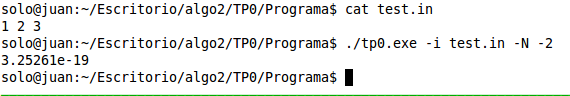
\includegraphics[scale=0.8]{prueba_fail_n_negativo.png}
		\label{graf:n_negativo}
		\caption{Corrida de prueba ante un valor de \texttt{n\_decimator} negativo}
	\end{figure}

\subsection{Índice de \texttt{n\_decimator} negativo}

	Como se ve en la Figura 12 el programa efectua algún tipo de operación a partir del número negativo. Como se ve en el código de la función \texttt{opt\_n\_decimator()} expuesto en la página 2 del presente informe, la variable \texttt{n\_decimator} almacena de forma directa el valor de entrada. Como ésta es una variable del tipo \texttt{size\_t}, al asignarle un valor negativo almacena el valor máximo representable menos el módulo de lo que se ingresó.

	Para su solución se agregó una variable auxiliar tipo \texttt{int}, para que almacene temporalmente el valor entrante con su signo y compruebe si es positivo. De serlo, se almacena dicho valor en la variable estática \texttt{n\_decimator}. A continuación se presenta la nueva implementación de la función y la corrida de prueba del nuevo programa:

	\begin{lstlisting}[frame=single]
static void
opt_n_decimator(string const &arg)
{
	istringstream iss(arg);
	int aux;

	// Intentamos extraer el N de la línea de comandos.
	// Para detectar argumentos que únicamente consistan de
	// números enteros, vamos a verificar que EOF llegue justo
	// después de la lectura exitosa del escalar.
	
	if(!(iss >> aux) || !iss.eof() || aux<0) {
		cerr << "non-positive integer factor: "
		     << arg
		     << "."
		     << endl;
		exit(1);
	}
	if (iss.bad()) {
		cerr << "cannot read integer factor."
		     << endl;
		exit(1);
	}
	n_decimator=aux;
}
	\end{lstlisting}

	\begin{figure}[H]
		\centering
		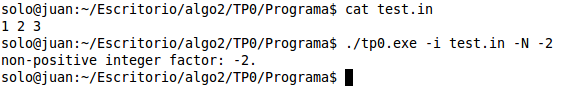
\includegraphics[scale=0.8]{prueba_ok_n_negativo.png}
		\label{graf:ok_n_negativo}
		\caption{Corrida satisfactoria de la prueba para \texttt{n\_decimator<0}}
	\end{figure}
	
\subsection{Prueba de memoria}

	Para el análisis de manejo de memoria del programa se utilizó el programa \texttt{valgrind} llamándolo de la siguiente forma:
		\begin{center}
			\texttt{valgrind --tool=memcheck ./tp0.exe>test\_valgrind.in}
		\end{center}
	
	El archivo \texttt{test\_valgrind.in} consta de 1000 números reales generados aleatoriamente. Éste fue el resultado:
		\begin{figure}[H]
			\centering
			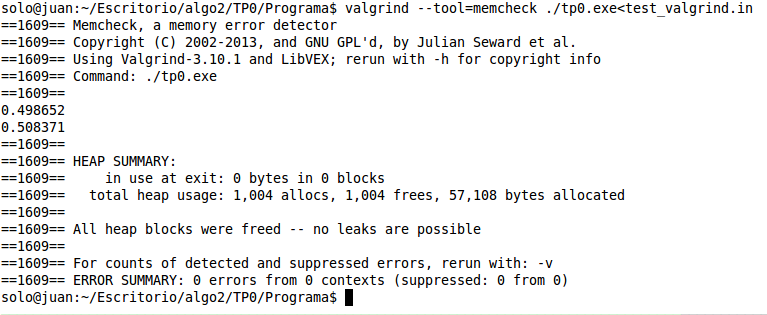
\includegraphics[scale=0.6]{prueba_valgrind.png}
			\label{graf:valgrind}
			\caption{Corrida del programa \texttt{tp0.exe} bajo el análisis del \texttt{valgrind}}
		\end{figure}
	
	Como se ve en la Figura 14 el manejo de memoria del programa es bueno, dado que al finalizar no fuga memoria.
